\subsection{User Journeys}

The below sequence diagrams show the interactions between the different entities. As part of the design process, the way in which these entities interact is fundamental to the implementation. The interactions between the patient and doctor are assumed to be non-digital (e.g. verbal). There is an assumption that the doctor has the ability to communicate with a local hospital for the purposes of referring treatment on a patient's behalf. The hospital has a 'data gateway' representing some host that has the ability to be communicated with via a RESTful API, and communicates with a patient's chain and off-chain storage directly. The 'data gateway' is intended as an extension to a hospital's current systems to allow the integration of modern technologies. The hospital is also assumed to have a direct connection to an authority to verify the validity of medical personnel, which for doctors is the GMC~\footnote{\href{http://www.gmc-uk.org/}{General Medical Council}}.

\subsubsection{Doctor requests X-ray}

\begin{figure}[H]
  \centering
  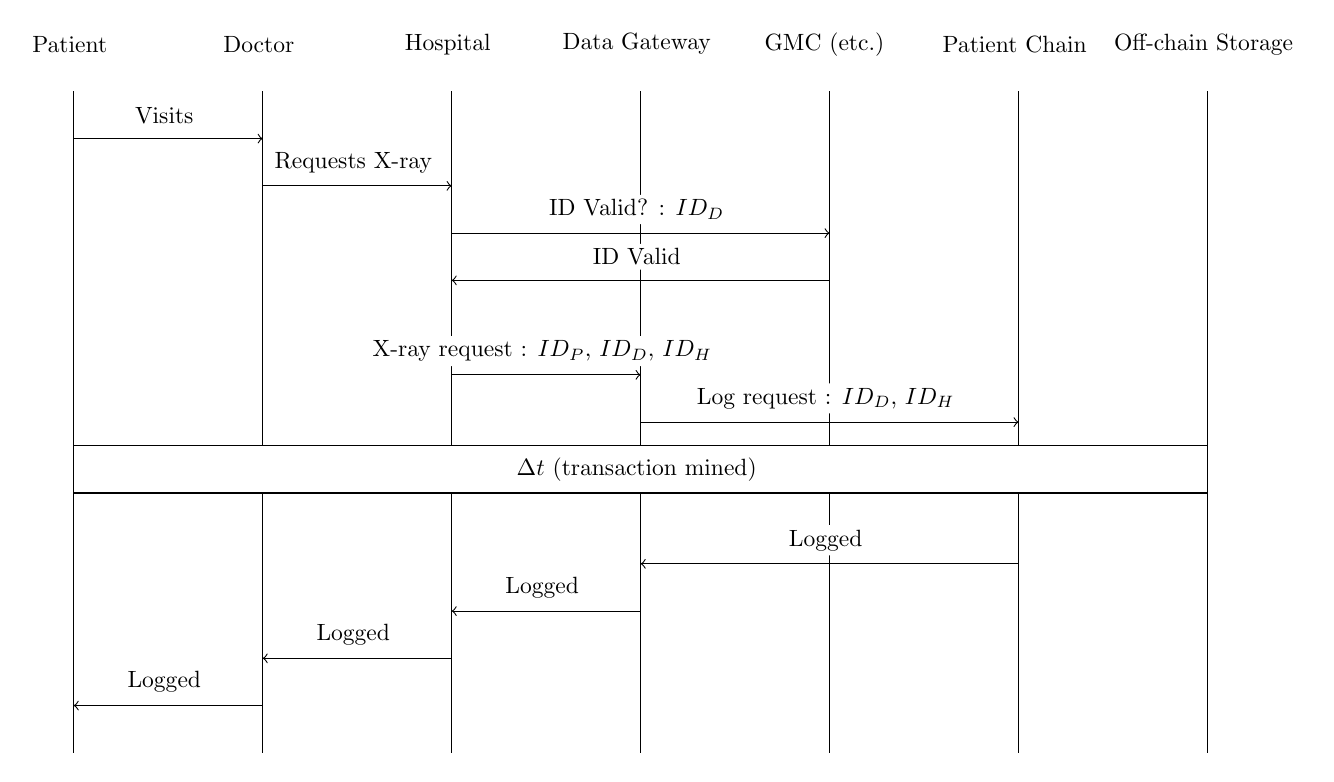
\begin{tikzpicture}[scale = 0.6, every node/.style={scale = 0.85}, every node/.append style={fill = white, rounded corners = 2pt, inner sep = 2pt, align = center}]

  % Lines
  \draw (4, 6) -- (4, 20);
  \draw (8, 6) -- (8, 20);
  \draw (12, 6) -- (12, 20);
  \draw (16, 6) -- (16, 20);
  \draw (20, 6) -- (20, 20);
  \draw (24, 6) -- (24, 20);
  \draw (28, 6) -- (28, 20);

  % Headings
  \node at (4, 21) { Patient };
  \node at (8, 21) { Doctor };
  \node at (12, 21) { Hospital };
  \node at (16, 21) { Data Gateway };
  \node at (20, 21) { GMC (etc.) };
  \node at (24, 21) { Patient Chain };
  \node at (28, 21) { Off-chain Storage };

  % Arrows
  \node at (6, 19.5) { Visits };
  \draw [ -> ] (4, 19) -- (8, 19);

  \node at (10, 18.5) { Requests X-ray };
  \draw [ -> ] (8, 18) -- (12, 18);

  \node at (16, 17.5) { ID Valid? : $ID_{D}$ };
  \draw [ -> ] (12, 17) -- (20, 17);

  \node at (16, 16.5) { ID Valid \checkmark };
  \draw [ -> ] (20, 16) -- (12, 16);

  \node at (14, 14.5) { X-ray request : $ID_{P}$, $ID_{D}$, $ID_{H}$ };
  \draw [ -> ] (12, 14) -- (16, 14);

  \node at (20, 13.5) { Log request : $ID_{D}$, $ID_{H}$ };
  \draw [ -> ] (16, 13) -- (24, 13);

  \draw[fill = white] (4, 12.5) rectangle (28, 11.5);
  \node at (16, 12) { $\Delta t$ (transaction mined) };

  \node at (20, 10.5) { Logged \checkmark };
  \draw [ -> ] (24, 10) -- (16, 10);

  \node at (14, 9.5) { Logged \checkmark };
  \draw [ -> ] (16, 9) -- (12, 9);

  \node at (10, 8.5) { Logged \checkmark };
  \draw [ -> ] (12, 8) -- (8, 8);

  \node at (6, 7.5) { Logged \checkmark };
  \draw [ -> ] (8, 7) -- (4, 7);

  \end{tikzpicture}
  \caption{
    Doctor requests that patient have X-ray taken
  }
  \label{fig:user_story_01}
\end{figure}


\subsubsection{Patient has X-ray taken}

\begin{figure}[H]
  \centering
  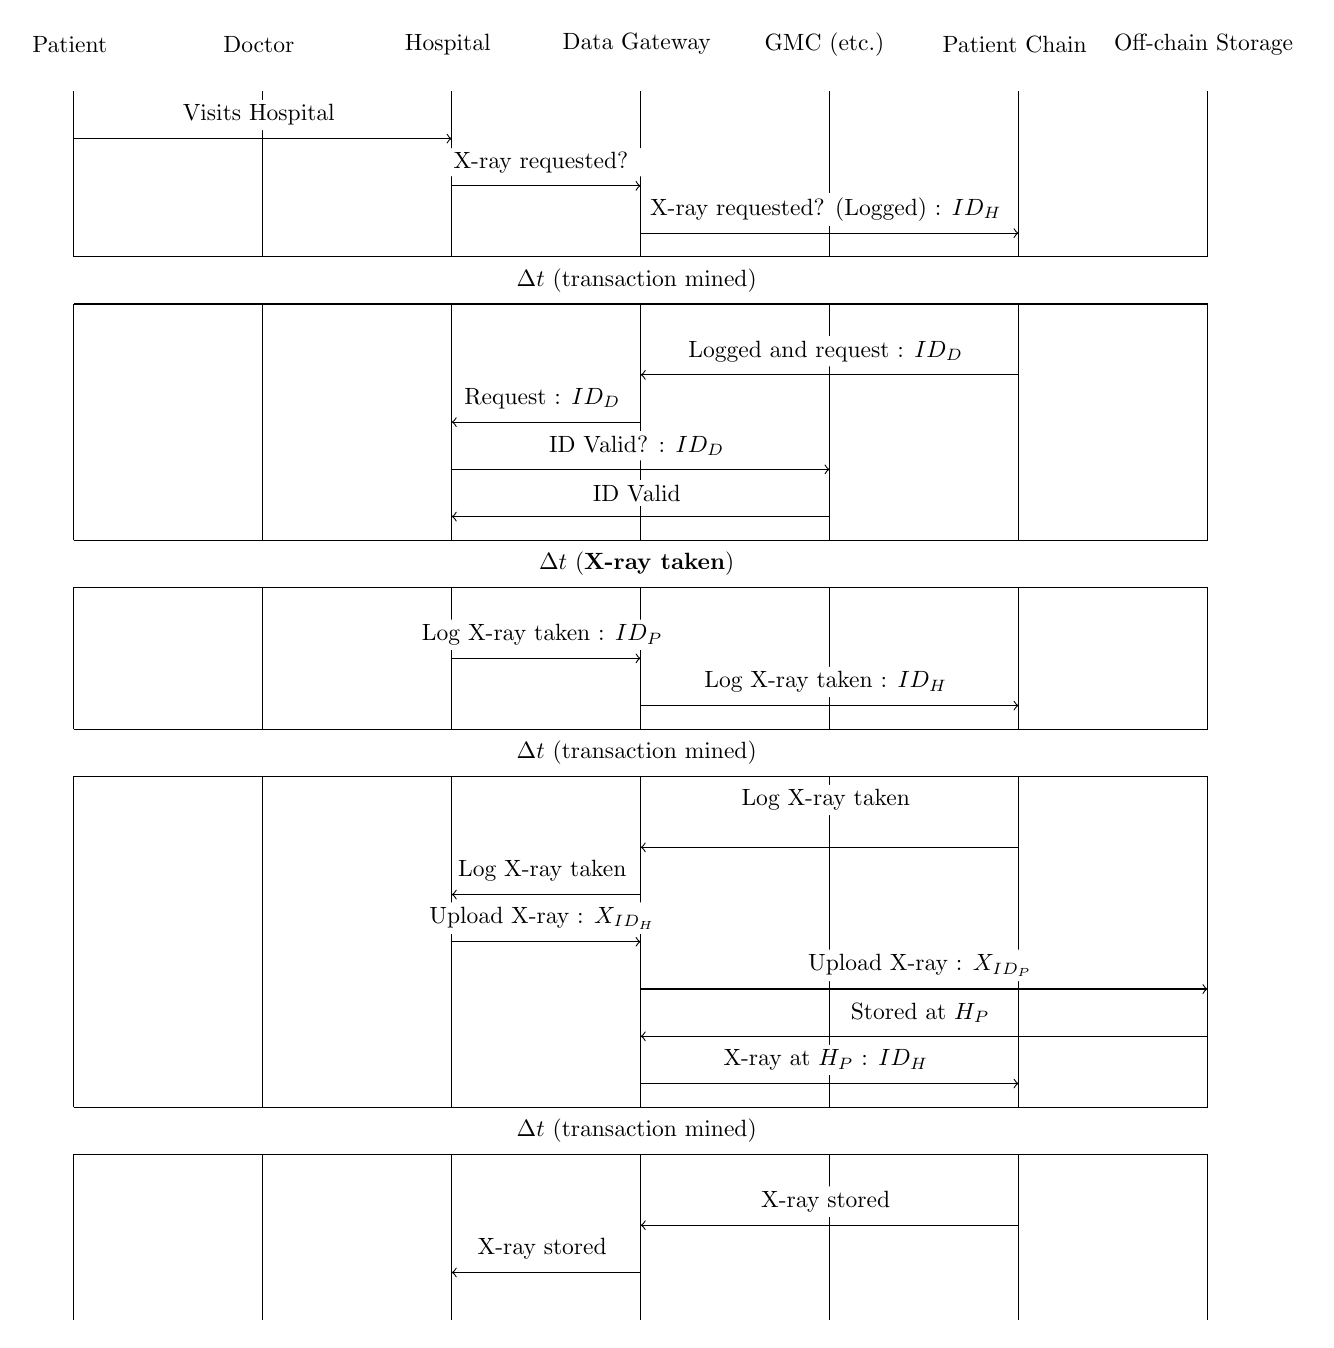
\begin{tikzpicture}[scale = 0.6, every node/.style={scale = 0.85}, every node/.append style={fill = white, rounded corners = 2pt, inner sep = 2pt, align = center}]

  % Lines
  \draw (4, -6) -- (4, -2.5);
  \draw (4, -1.5) -- (4, 5.5);
  \draw (4, 6.5) -- (4, 9.5);
  \draw (4, 10.5) -- (4, 15.5);
  \draw (4, 16.5) -- (4, 20);
  \draw (8, -6) -- (8, -2.5);
  \draw (8, -1.5) -- (8, 5.5);
  \draw (8, 6.5) -- (8, 9.5);
  \draw (8, 10.5) -- (8, 15.5);
  \draw (8, 16.5) -- (8, 20);
  \draw (12, -6) -- (12, -2.5);
  \draw (12, -1.5) -- (12, 5.5);
  \draw (12, 6.5) -- (12, 9.5);
  \draw (12, 10.5) -- (12, 15.5);
  \draw (12, 16.5) -- (12, 20);
  \draw (16, -6) -- (16, -2.5);
  \draw (16, -1.5) -- (16, 5.5);
  \draw (16, 6.5) -- (16, 9.5);
  \draw (16, 10.5) -- (16, 15.5);
  \draw (16, 16.5) -- (16, 20);
  \draw (20, -6) -- (20, -2.5);
  \draw (20, -1.5) -- (20, 5.5);
  \draw (20, 6.5) -- (20, 9.5);
  \draw (20, 10.5) -- (20, 15.5);
  \draw (20, 16.5) -- (20, 20);
  \draw (24, -6) -- (24, -2.5);
  \draw (24, -1.5) -- (24, 5.5);
  \draw (24, 6.5) -- (24, 9.5);
  \draw (24, 10.5) -- (24, 15.5);
  \draw (24, 16.5) -- (24, 20);
  \draw (28, -6) -- (28, -2.5);
  \draw (28, -1.5) -- (28, 5.5);
  \draw (28, 6.5) -- (28, 9.5);
  \draw (28, 10.5) -- (28, 15.5);
  \draw (28, 16.5) -- (28, 20);

  % Headings
  \node at (4, 21) { Patient };
  \node at (8, 21) { Doctor };
  \node at (12, 21) { Hospital };
  \node at (16, 21) { Data Gateway };
  \node at (20, 21) { GMC (etc.) };
  \node at (24, 21) { Patient Chain };
  \node at (28, 21) { Off-chain Storage };

  % Arrows
  \node at (8, 19.5) { Visits Hospital };
  \draw [ -> ] (4, 19) -- (12, 19);

  \node at (14, 18.5) { X-ray requested? };
  \draw [ -> ] (12, 18) -- (16, 18);

  \node at (20, 17.5) { X-ray requested? (Logged) : $ID_{H}$ };
  \draw [ -> ] (16, 17) -- (24, 17);

  \draw (4, 16.5) -- (28, 16.5);
  \node at (16, 16) { $\Delta t$ (transaction mined) };
  \draw (4, 15.5) -- (28, 15.5);

  \node at (20, 14.5) { Logged \checkmark and request : $ID_{D}$ };
  \draw [ -> ] (24, 14) -- (16, 14);

  \node at (14, 13.5) { Request : $ID_{D}$ };
  \draw [ -> ] (16, 13) -- (12, 13);

  \node at (16, 12.5) { ID Valid? : $ID_{D}$ };
  \draw [ -> ] (12, 12) -- (20, 12);

  \node at (16, 11.5) { ID Valid \checkmark };
  \draw [ -> ] (20, 11) -- (12, 11);

  \draw (4, 10.5) -- (28, 10.5);
  \node at (16, 10) { $\Delta t$ (\textbf{X-ray taken}) };
  \draw (4, 9.5) -- (28, 9.5);

  \node at (14, 8.5) { Log X-ray taken : $ID_{P}$ };
  \draw [ -> ] (12, 8) -- (16, 8);

  \node at (20, 7.5) { Log X-ray taken : $ID_{H}$ };
  \draw [ -> ] (16, 7) -- (24, 7);

  \draw (4, 6.5) -- (28, 6.5);
  \node at (16, 6) { $\Delta t$ (transaction mined) };
  \draw (4, 5.5) -- (28, 5.5);

  \node at (20, 5) { Log X-ray taken \checkmark };
  \draw [ -> ] (24, 4) -- (16, 4);

  \node at (14, 3.5) { Log X-ray taken \checkmark };
  \draw [ -> ] (16, 3) -- (12, 3);

  \node at (14, 2.5) { Upload X-ray : $X_{ID_{H}}$ };
  \draw [ -> ] (12, 2) -- (16, 2);

  \node at (22, 1.5) { Upload X-ray : $X_{ID_{P}}$ };
  \draw [ -> ] (16, 1) -- (28, 1);

  \node at (22, 0.5) { Stored at $H_{P}$ };
  \draw [ -> ] (28, 0) -- (16, 0);

  \node at (20, -0.5) { X-ray at $H_{P}$ : $ID_{H}$ };
  \draw [ -> ] (16, -1) -- (24, -1);

  \draw (4, -1.5) -- (28, -1.5);
  \node at (16, -2) { $\Delta t$ (transaction mined) };
  \draw (4, -2.5) -- (28, -2.5);

  \node at (20, -3.5) { X-ray stored \checkmark };
  \draw [ -> ] (24, -4) -- (16, -4);

  \node at (14, -4.5) { X-ray stored \checkmark };
  \draw [ -> ] (16, -5) -- (12, -5);

  \end{tikzpicture}
  \caption{
    Patient visits hospital to have X-ray taken
  }
  \label{fig:user_story_02}
\end{figure}


\subsubsection{Doctor views (and discusses) X-ray}

\begin{figure}[H]
  \centering
  \begin{tikzpicture}[scale = 0.6, every node/.style={scale = 0.85}, every node/.append style={fill = white, rounded corners = 2pt, inner sep = 2pt, align = center}]

  % Lines
  \draw (4, 2) -- (4, 20);
  \draw (8, 2) -- (8, 20);
  \draw (12, 2) -- (12, 20);
  \draw (20, 2) -- (20, 20);
  \draw (24, 2) -- (24, 20);
  \draw (28, 2) -- (28, 20);

  % Headings
  \node at (4, 21) { Patient };
  \node at (8, 21) { Doctor };
  \node at (12, 21) { Hospital };
  \node at (20, 21) { GMC (etc.) };
  \node at (24, 21) { Patient Chain };
  \node at (28, 21) { Off-chain Storage };

  % Arrows
  \node at (6, 19.5) { Visits };
  \draw [ -> ] (4, 19) -- (8, 19);

  \node at (16, 18.5) { Get X-ray address : $ID_{D}$ };
  \draw [ -> ] (8, 18) -- (24, 18);

  \node at (22, 17.5) { ID Valid? : $ID_{D}$ };
  \draw [ -> ] (24, 17) -- (20, 17);

  \node at (22, 16.5) { ID Valid \checkmark };
  \draw [ -> ] (20, 16) -- (24, 16);

  \node at (16, 15.5) { X-ray address : $H_{\text{X-ray}} };
  \draw [ -> ] (24, 15) -- (8, 15);

  \node at (18, 14.5) { Get X-ray Data : $H_{\text{X-ray}} };
  \draw [ -> ] (8, 14) -- (28, 14);

  \node at (20, 14.5) { X-ray stored \checkmark : $H_{\text{X-ray}}$ };
  \draw [ -> ] (28, 14) -- (12, 14);

  \node at (31, 13) { \textit{Transaction starts} };
  \draw [ dashed ] (4, 13) -- (28, 13);

  \node at (18, 12.5) { Add X-ray Data : $H_{\text{X-ray}}$, $ID_{H}$ };
  \draw [ -> ] (12, 12) -- (24, 12);

  \node at (22, 11.5) { ID Valid? : $ID_{H}$ };
  \draw [ -> ] (24, 11) -- (20, 11);

  \node at (22, 10.5) { ID Valid \checkmark };
  \draw [ -> ] (20, 10) -- (24, 10);

  \node at (18, 9.5) { Request success };
  \draw [ -> ] (24, 9) -- (12, 9);

  \node at (31, 8) { \textit{Transaction ends} };
  \draw [ dashed ] (4, 8) -- (28, 8);

  \end{tikzpicture}
  \caption{Doctor views X-ray with patient}{
  	The patient visits the doctor to discuss their X-ray results. The doctor gets the latest version (address / hash) of their X-ray data from their record and using this gets the X-ray data itself from off-chain storage. The doctor is then able to discuss the results with the patient (and make further edits - \textit{not shown}.
  }
  \label{fig:user_story_03}
\end{figure}


\subsubsection{Patient views their log}

\begin{figure}[H]
  \centering
  \begin{tikzpicture}[scale = 0.6, every node/.style={scale = 0.85}, every node/.append style={fill = white, rounded corners = 2pt, inner sep = 2pt, align = center} ]

  % Lines
  \draw (4, 4) -- (4, 20);
  \draw (8, 4) -- (8, 20);
  \draw (12, 4) -- (12, 20);
  \draw (16, 4) -- (16, 20);
  \draw (20, 4) -- (20, 20);
  \draw (24, 4) -- (24, 20);
  \draw (28, 4) -- (28, 20);

  % Headings
  \node at (4, 21) { Patient };
  \node at (8, 21) { Doctor };
  \node at (12, 21) { Hospital };
  \node at (16, 21) { Data Gateway };
  \node at (20, 21) { GMC (etc.) };
  \node at (24, 21) { Patient Chain };
  \node at (28, 21) { Off-chain Storage };

  % Arrows
  \node at (10, 19.5) { Requests Log };
  \draw [ -> ] (4, 19) -- (16, 19);

  \node at (20, 18.5) { Log request for Log : $ID_{H}$, $ID_{P}$ };
  \draw [ -> ] (16, 18) -- (24, 18);

  \draw[fill = white] (4, 17.5) rectangle (28, 16.5);
  \node at (16, 17) { $\Delta t$ (transaction mined) };

  \node at (20, 15.5) { Logged \checkmark };
  \draw [ -> ] (24, 15) -- (16, 15);

  \node at (20, 14.5) { Retrieve log };
  \draw [ -> ] (16, 14) -- (24, 14);

  \node at (20, 13.5) { Log Data };
  \draw [ -> ] (24, 13) -- (16, 13);

  \node at (10, 12.5) { Log Data };
  \draw [ -> ] (16, 12) -- (4, 12);

  \end{tikzpicture}
  \caption{
    Patient retrieves log of accesses to their account and also appends their own access in the process by using a centralised data gateway
  }
  \label{fig:user_story_04a}
\end{figure}


\begin{figure}[H]
  \centering
  \begin{tikzpicture}[scale = 0.6, every node/.style={scale = 0.85}]

  % Lines
  \draw (4, 4) -- (4, 20);
  \draw (8, 4) -- (8, 20);
  \draw (12, 4) -- (12, 20);
  \draw (16, 4) -- (16, 20);
  \draw (20, 4) -- (20, 20);
  \draw (24, 4) -- (24, 20);
  \draw (28, 4) -- (28, 20);

  % Headings
  \node[fill = white, rounded corners = 2pt, inner sep = 2pt, align = center] at (4, 21) { Patient };
  \node[fill = white, rounded corners = 2pt, inner sep = 2pt, align = center] at (8, 21) { Doctor };
  \node[fill = white, rounded corners = 2pt, inner sep = 2pt, align = center] at (12, 21) { Hospital };
  \node[fill = white, rounded corners = 2pt, inner sep = 2pt, align = center] at (16, 21) { Data Gateway };
  \node[fill = white, rounded corners = 2pt, inner sep = 2pt, align = center] at (20, 21) { GMC (etc.) };
  \node[fill = white, rounded corners = 2pt, inner sep = 2pt, align = center] at (24, 21) { Patient Chain };
  \node[fill = white, rounded corners = 2pt, inner sep = 2pt, align = center] at (28, 21) { Off-chain Storage };

  \end{tikzpicture}
  \caption{
    Doctor requests that patient have X-ray taken
  }
  \label{fig:user_story_04}
\end{figure}

